\chapter{Stationary Action and the Euler--Lagrange Equation}

The lecture begins with a correction that is more than verbal. We are told that the phrase ``principle of least action'' is a misnomer: the essential word is not ``least'' but ``stationary.'' Susskind does not define the action at once. He first retreats to the simpler problem of equilibrium, where stationarity can be understood for an ordinary potential energy. Only after that does he move to whole trajectories, to the calculus of variations, and finally to the action itself. The order matters. We learn first what it means for a quantity not to change at first order, and only then do we ask for a whole path in spacetime to have that property.

\section{Stationary, Not Necessarily Least}

Let us begin where the lecture begins: with equilibrium. If a system is at rest, then in the ordinary Newtonian language the force vanishes. When the force comes from a potential energy \(V\), the equilibrium condition can be written, for one coordinate \(x\), as
\begin{equation}
\frac{dV(x)}{dx}=0.
\end{equation}

\begin{figure}[h]
\centering

\includegraphics[width=0.68\textwidth]{lecture_03_figure_02.png}
\caption{Stationary point condition for the potential. The board is still open below the equation, anticipating the geometric discussion in terms of the graph of \(V(x)\).}
\end{figure}

The point of the opening is that this does \emph{not} mean the potential must be minimal. A derivative can vanish at a minimum, at a maximum, or, in more than one dimension, at a saddle point. What stationarity means is simply that the first derivative vanishes.

This is already visible if we think in terms of a small displacement. If we move the particle by a small amount \(\delta x\), then the first-order change in the potential is
\begin{equation}
\delta V=\frac{dV}{dx}\,\delta x.
\end{equation}
At equilibrium this first-order change is zero:
\begin{equation}
\delta V=0.
\end{equation}
That is the first appearance of the variational language, and it is worth pausing over it. The condition is not that the potential fails to change \emph{exactly}; it is that the change vanishes to first order in a small displacement.

\begin{figure}[h]
\centering
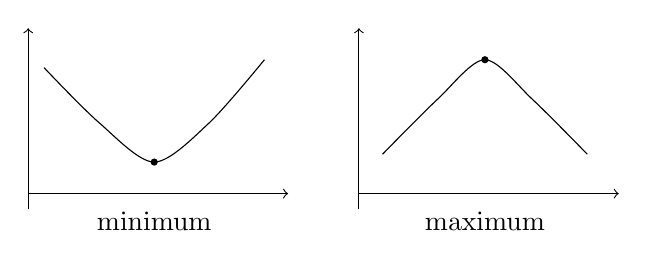
\begin{tikzpicture}[scale=1.0]
\draw[->] (0,-0.1) -- (3.3,-0.1);
\draw[->] (0,-0.3) -- (0,2.0);
\draw[smooth] plot coordinates {(0.2,1.5) (0.9,0.8) (1.6,0.3) (2.3,0.8) (3.0,1.6)};
\fill (1.6,0.3) circle (1.3pt);
\node at (1.6,-0.45) {minimum};

\draw[->] (4.2,-0.1) -- (7.5,-0.1);
\draw[->] (4.2,-0.3) -- (4.2,2.0);
\draw[smooth] plot coordinates {(4.5,0.4) (5.2,1.1) (5.8,1.6) (6.4,1.1) (7.1,0.4)};
\fill (5.8,1.6) circle (1.3pt);
\node at (5.8,-0.45) {maximum};
\end{tikzpicture}
\caption{Two one-dimensional stationary points. In one dimension the derivative vanishes at minima and maxima alike.}
\end{figure}

In more than one coordinate the same logic remains, but now the geometry becomes richer. Suppose \(V\) depends on \(x\) and \(y\). Then the first-order change under an infinitesimal displacement \((\delta x,\delta y)\) is
\begin{equation}
\delta V=\frac{\partial V}{\partial x}\,\delta x+\frac{\partial V}{\partial y}\,\delta y.
\end{equation}
For many coordinates this becomes
\begin{equation}
\delta V=\sum_i \frac{\partial V}{\partial x_i}\,\delta x_i.
\end{equation}
If \(\delta V\) must vanish for \emph{every} infinitesimal displacement, then each coefficient must vanish:
\begin{equation}
\frac{\partial V}{\partial x_i}=0 \qquad \text{for every } i.
\end{equation}

Now we see why Susskind insists so strongly on the word stationary. In many dimensions the generic stationary point is often not a minimum and not a maximum, but a saddle. In one direction you climb uphill, in another you roll down. Yet precisely at the saddle the first-order change still vanishes in every direction. That is all stationarity means, and that is the idea we are going to transport from ordinary functions to whole trajectories.

\section{From Points to Functions}

Now of course we are not interested only in equilibrium. We are interested in whole motions, and before we get to mechanics Susskind wants the variational pattern to appear in simpler settings.

The simplest example is the shortest path between two fixed points in the plane. Let the path be given by a function \(y(x)\). If we move a short distance \(dx\) horizontally and \(dy\) vertically, the length of the little segment of the curve is
\begin{equation}
ds=\sqrt{dx^2+dy^2}=dx\,\sqrt{1+\left(\frac{dy}{dx}\right)^2}.
\end{equation}
Therefore the total length of the curve is
\begin{equation}
S[y]=\int ds=\int dx\,\sqrt{1+\left(\frac{dy}{dx}\right)^2}.
\end{equation}
The problem is not yet to solve the integral, but to understand the structure of the question: among all functions \(y(x)\) that pass through the two endpoints, which one makes this quantity stationary? In the language we have just learned,
\begin{equation}
\delta S=0.
\end{equation}

Susskind immediately enlarges the example. On a curved surface the same question defines a geodesic. The shortest path is no longer a straight line, but the logic is unchanged: fixed endpoints, an integral built from little distance elements, and the requirement that the total be stationary.

The same structure appears again in Fermat's principle. If light moves through a medium whose speed \(c(x,y)\) depends on position, then the time to travel along a small segment is the distance divided by the local speed. Thus
\begin{equation}
T[y]=\int dx\,\frac{\sqrt{1+\left(\frac{dy}{dx}\right)^2}}{c(x,y)}.
\end{equation}
Here too the path is chosen by a variational condition:
\begin{equation}
\delta T=0.
\end{equation}
If \(c\) is constant, least time reduces to least distance. But when the speed varies, the path of light is not determined by geometry alone; it is determined by the geometry \emph{and} the medium. That is an important warning for what will come later in mechanics: the integrand will generally depend not only on position but also on derivatives.

Before turning to action, Susskind inserts one more example: the hanging chain. A chain pinned at two points settles into a shape that makes its potential energy stationary. Again, the endpoints are fixed, the shape is a function, and the quantity to be stationarized is an integral over the curve.

\begin{figure}[h]
\centering

\includegraphics[width=0.70\textwidth]{lecture_03_figure_03.png}
\caption{Suspended stationary curve between fixed endpoints. The figure is diagrammatic rather than symbolic; its value is to preserve the fixed-endpoint geometry on the board.}
\end{figure}

\begin{figure}[h]
\centering
\begin{tikzpicture}[scale=1.1]
\fill (0,2.1) circle (1.5pt);
\fill (4.6,2.2) circle (1.5pt);
\draw[smooth] plot coordinates {(0,2.1) (0.9,1.2) (1.8,0.75) (2.8,0.85) (3.8,1.3) (4.6,2.2)};
\end{tikzpicture}
\caption{A cleaned schematic of the same fixed-endpoint variational problem. The lecture uses it as one last reminder that the basic pattern is: two fixed endpoints, one function in between, one integral to be made stationary.}
\end{figure}

By this point the recurring motif is unmistakable. We keep the endpoints fixed, we write down some integral quantity in between, and we ask for that quantity to be stationary under small changes of the curve. The only thing missing is mechanics itself.

\section{Mechanics Recast as a Problem of Whole Trajectories}

We now turn from curves in space to curves in spacetime. A mechanical trajectory is a function such as \(x(t)\), or in more dimensions \(x(t)\), \(y(t)\), \(z(t)\). Susskind briefly contrasts two formulations of mechanics.

In the usual initial-value formulation we specify the initial position and the initial velocity, and Newton's equations build the orbit forward. But there is another way to pose the problem. We may specify the position at an initial time \(t_0\) and the position at a later time \(t_1\), and ask which path between them is the actual one. Then the initial velocity is not input data; it becomes part of the solution.

This is the moment when the action enters. For a trajectory between fixed times \(t_0\) and \(t_1\), we define
\begin{equation}
A=\int_{t_0}^{t_1} L(x,\dot x,t)\,dt.
\end{equation}
The function \(L\) is the Lagrangian. Along the path it depends on position and on velocity, and in general it may depend on time as well. The mechanical question is now cast in the same language as the earlier variational problems: among all trajectories connecting the two endpoint events, which one makes the action stationary?

This is not yet a differential equation. It is a global statement about an integral over a whole path. So the next question arises exactly where it should: how can such a statement possibly turn into something that looks like Newton's local equations of motion?

\section{The Euler--Lagrange Equation from a Discretized Path}

The lecture answers that question in a deliberately concrete way. We do not begin with a polished proof. We first approximate the curve by a broken line.

To avoid an index collision with the later many-coordinate notation, let us label the discrete time-slices by \(n\). Divide the interval from \(t_0\) to \(t_1\) into steps of size \(\epsilon\), and let \(x_n\) be the position at the \(n\)-th time. Then the velocity on the interval from \(n\) to \(n+1\) is approximated by
\begin{equation}
v_n \approx \frac{x_{n+1}-x_n}{\epsilon}.
\end{equation}
The action integral is then approximated by an ordinary sum,
\begin{equation}
A_\epsilon=\sum_{n=0}^{N-1}\epsilon\,L\!\left(x_n,\frac{x_{n+1}-x_n}{\epsilon}\right).
\end{equation}

This is the bridge. We have replaced a functional of a curve by an ordinary function of finitely many variables \(x_0,x_1,\dots,x_N\). Stationarity can now be imposed by differentiating with respect to those variables.

Pick one interior point \(x_n\), and vary it while holding all the others fixed. Then only the two neighboring intervals change. That is the local mechanism behind the whole derivation. The action depends on \(x_n\) through the interval in front and the interval behind, and nowhere else. If we differentiate with respect to \(x_n\), we find
\begin{align}
0
&=\frac{\partial A_\epsilon}{\partial x_n} \\
&=\epsilon\,\frac{\partial L_n}{\partial x_n}
-\frac{\partial L_n}{\partial v_n}
+\frac{\partial L_{n-1}}{\partial v_{n-1}},
\end{align}
where \(L_n\) is shorthand for
\[
L_n=L\!\left(x_n,\frac{x_{n+1}-x_n}{\epsilon}\right).
\]
Rearranging,
\begin{equation}
\frac{1}{\epsilon}
\left(
\frac{\partial L_n}{\partial v_n}
-
\frac{\partial L_{n-1}}{\partial v_{n-1}}
\right)
=
\frac{\partial L_n}{\partial x_n}.
\end{equation}

Now the crucial observation is exactly the one Susskind emphasizes aloud: the difference of two neighboring values of a function, divided by \(\epsilon\), becomes a derivative when \(\epsilon\) is small. Thus, in the continuum limit,
\begin{equation}
\frac{d}{dt}\!\left(\frac{\partial L}{\partial \dot x}\right)=\frac{\partial L}{\partial x}.
\end{equation}
This is the Euler--Lagrange equation.

\begin{figure}[h]
\centering

\includegraphics[width=0.62\textwidth]{lecture_03_figure_04.png}
\caption{Derivative terms in the Euler--Lagrange construction. The board clearly separates the position derivative from the velocity-derivative structure, even though the intermediate finite-difference details are only partly legible.}
\end{figure}

The board evidence at this stage is partial, so it is better to state the cleaned result than to pretend every intermediate symbol is readable. But the logic is faithful to the lecture: vary one interior point, watch only the two neighboring intervals change, and the time derivative emerges from a neighboring difference quotient.

Susskind's next remark is pedagogically important. Once the Lagrangian is given, the Euler--Lagrange equation is a kind of machine. Feed in \(L\), and out comes the differential equation of motion.

\section{Recovering Newton's Equations}

A machine is only interesting if it reproduces something we already trust. So Susskind now tests it on the familiar case of a particle moving in a potential.

For one coordinate, take
\begin{equation}
L=\frac{1}{2}m\dot x^2 - V(x).
\end{equation}
Then
\begin{equation}
\frac{\partial L}{\partial \dot x}=m\dot x,
\end{equation}
and therefore
\begin{equation}
\frac{d}{dt}\!\left(\frac{\partial L}{\partial \dot x}\right)=m\ddot x.
\end{equation}
On the other hand,
\begin{equation}
\frac{\partial L}{\partial x}=-\frac{dV}{dx}.
\end{equation}
Putting these into the Euler--Lagrange equation gives
\begin{equation}
m\ddot x=-\frac{dV}{dx}.
\end{equation}
That is precisely Newton's law for a force derived from a potential:
\begin{equation}
F(x)=-\frac{dV}{dx}.
\end{equation}

At this point Susskind also pauses over a definition that will recur throughout mechanics: \(\partial L/\partial \dot x\) is the momentum. Here it is just \(m\dot x\), but the important point is that this becomes the general Lagrangian definition of momentum.

\begin{figure}[h]
\centering

\includegraphics[width=0.74\textwidth]{lecture_03_figure_05.png}
\caption{Lagrangian as kinetic minus potential energy. The board mixes one-coordinate and indexed notation, but its summary structure is clear: potential energy, kinetic energy, \(L=T-V\), and Newton's force law in one view.}
\end{figure}

For many particles and many coordinates, the extension is straightforward. If the kinetic energy is
\begin{equation}
T=\sum_i \frac{m_i}{2}\dot x_i^{\,2},
\end{equation}
and the potential is \(V(x_1,x_2,\dots)\), then
\begin{equation}
L=T-V
\end{equation}
leads to one Euler--Lagrange equation for each coordinate,
\begin{equation}
m_i\ddot x_i=-\frac{\partial V}{\partial x_i}=F_i.
\end{equation}
The trajectory through configuration space is still a single curve, but now the curve lives in a higher-dimensional space.

\subsection{Question \& Answer}

\paragraph{Question.} Why is the Lagrangian \(T-V\) rather than \(T+V\)?

\paragraph{Answer.} Because with the force convention already in place, \(F_i=-\partial V/\partial x_i\), the plus sign would give the wrong Newtonian equation. If we wrote \(L=T+V\), then the Euler--Lagrange equation would produce
\[
m_i\ddot x_i=+\frac{\partial V}{\partial x_i}=-F_i,
\]
so mass times acceleration would come out equal to minus the force. One could rescue that only by redefining force or redefining potential energy. With the standard definitions already used throughout mechanics, the Lagrangian must be kinetic energy minus potential energy.

There is a second point hidden inside the same question. The Lagrangian is not the total energy. That is why it need not be \(T+V\). It is a different object, chosen so that the stationarity of the action reproduces the equations of motion.

\section{The Lagrangian as Packaging}

At this stage the lecture raises a natural resistance point. Have we merely worked backward from Newton's equations, selecting a convenient functional only because we already knew the answer?

\subsection{Question \& Answer}

\paragraph{Question.} Does the action principle merely work backward from the answer?

\paragraph{Answer.} Susskind's answer is no, and it is worth preserving the force of that answer. The useful point of view is not that we begin with Newton's equations and then engineer a Lagrangian to imitate them. The more powerful point of view is that the Lagrangian is itself the compact specification of the system. One function of all the coordinates and velocities packages the whole mechanics. From that one function the Euler--Lagrange equations extract the equations of motion.

This is how physicists typically think when proposing new laws. One does not usually guess the equations of motion directly. One guesses the action or the Lagrangian, because it is a simpler and more economical object.

That economy is the first reason the formalism is useful. The second is that the action principle is much friendlier to coordinate changes than Newton's equations written out component by component. A shortest path is shortest in any coordinate system. A straight line in the plane is still the shortest path whether we describe the plane by Cartesian coordinates, polar coordinates, or some more elaborate curvilinear system. The same is true of the action principle. The coordinate description changes, but the stationary character of the action does not.

This is the hinge that opens the final part of the lecture. Once we take the Lagrangian seriously as the given object, changing coordinates becomes natural rather than painful.

\section{Changing Coordinates: Rotating Frames and Polar Coordinates}

\subsection{Rotating coordinates}

Susskind's first example is a free particle, but viewed from a rotating coordinate system. In an inertial frame with Cartesian coordinates \((x,y)\), the Lagrangian is just
\begin{equation}
L_{\mathrm{inertial}}=\frac{m}{2}\left(\dot x^2+\dot y^2\right).
\end{equation}
Now introduce a second coordinate system \((X,Y)\) that rotates uniformly with angular velocity \(\omega\). The coordinate transformation used in the lecture is
\begin{equation}
\begin{aligned}
x&=X\cos\omega t+Y\sin\omega t,\\
y&=-X\sin\omega t+Y\cos\omega t.
\end{aligned}
\end{equation}

\begin{figure}[h]
\centering
\begin{tikzpicture}[scale=1.0]
\draw[->] (0,0) -- (2.6,0) node[right] {$x$};
\draw[->] (0,0) -- (0,2.6) node[above] {$y$};
\draw[->,dashed] (0,0) -- (2.1,1.0) node[right] {$X$};
\draw[->,dashed] (0,0) -- (-1.0,2.1) node[above] {$Y$};
\draw (0.8,0) arc (0:25:0.8);
\node at (1.0,0.28) {$\omega t$};
\end{tikzpicture}
\caption{A rotating coordinate frame. The lecture's point is that it is easier to transform the Lagrangian than to rewrite Newton's equations directly in these time-dependent coordinates.}
\end{figure}

One differentiates these relations, substitutes into \(\dot x^2+\dot y^2\), and simplifies. The lecture does not dwell on the algebra, and the transcript is noisy in the middle of it, so the clean thing to record is the standard reconstructed result:
\begin{equation}
\begin{aligned}
L_{\mathrm{rot}}
&=
\frac{m}{2}\left(\dot X^2+\dot Y^2\right)
+
\frac{m\omega^2}{2}\left(X^2+Y^2\right)\\
&\qquad
+ m\omega(\dot X\,Y-\dot Y\,X).
\end{aligned}
\end{equation}

The first term looks ordinary enough. The second has the form of minus a potential energy:
\begin{equation}
V_{\mathrm{fict}}=-\frac{m\omega^2}{2}\left(X^2+Y^2\right).
\end{equation}
Because this potential falls away outward from the origin, it produces an outward force. This is the centrifugal force.

The third term is different. It is linear both in coordinates and in velocities. That is exactly the kind of term that produces a velocity-dependent force. In the present context that force is the Coriolis force. Cleaning up the lecture's board-level sign slips, the corresponding equations of motion take the standard form
\begin{equation}
m\ddot X=m\omega^2 X-2m\omega \dot Y,
\qquad
m\ddot Y=m\omega^2 Y+2m\omega \dot X.
\end{equation}
The terms proportional to \(\omega^2\) are centrifugal. The terms proportional to the transverse velocity are Coriolis.

The conceptual point is more important than the algebraic details. A complicated transformation of Newton's equations is replaced by a comparatively painless transformation of the Lagrangian. Once the transformed Lagrangian is in hand, the Euler--Lagrange machine does the rest.

Susskind also remarks that the mixed term is not peculiar to rotating systems. A charged particle in a magnetic field is described by a very similar velocity-dependent contribution to the Lagrangian. That observation is a hint of a broader pattern: linear-in-velocity terms are natural in the Lagrangian language even when they look unfamiliar from the Newtonian point of view.

We also keep the energy discussion modest here, as the lecture does. The mixed linear term affects the equations of motion, but the fuller and more systematic treatment of energy is postponed to the Hamiltonian formulation.

\subsection{Polar coordinates and cyclic coordinates}

The next example is cleaner. Rewrite the same two-dimensional mechanics in ordinary polar coordinates:
\begin{equation}
x=r\cos\theta,
\qquad
y=r\sin\theta.
\end{equation}
Differentiating and squaring, one finds the familiar identity
\begin{equation}
\dot x^2+\dot y^2=\dot r^2+r^2\dot\theta^2.
\end{equation}
Thus the kinetic energy becomes
\begin{equation}
T=\frac{m}{2}\left(\dot r^2+r^2\dot\theta^2\right).
\end{equation}
For a central force, where the potential depends only on \(r\), the Lagrangian is
\begin{equation}
L=\frac{m}{2}\left(\dot r^2+r^2\dot\theta^2\right)-V(r).
\end{equation}

\begin{figure}[h]
\centering
\begin{tikzpicture}[scale=1.0]
\draw[->] (-0.2,0) -- (3.2,0) node[right] {$x$};
\draw[->] (0,-0.2) -- (0,2.6) node[above] {$y$};
\draw[->,thick] (0,0) -- (2.4,1.6);
\fill (2.4,1.6) circle (1.3pt);
\draw (0.8,0) arc (0:34:0.8);
\node at (1.05,0.25) {$\theta$};
\node at (1.35,1.0) {$r$};
\end{tikzpicture}
\caption{Polar coordinates for a central-force problem. The geometry makes the radial and angular equations easy to read.}
\end{figure}

Now the Euler--Lagrange equations are taken with respect to \(r\) and \(\theta\). For the radial coordinate,
\begin{equation}
\frac{d}{dt}\!\left(\frac{\partial L}{\partial \dot r}\right)=\frac{\partial L}{\partial r},
\end{equation}
so
\begin{equation}
m\ddot r=mr\dot\theta^2-\frac{dV}{dr}.
\end{equation}
The first term on the right is the familiar outward centrifugal contribution; here it comes not from rotating coordinates, but from the particle's own angular motion.

For the angular coordinate,
\begin{equation}
\frac{d}{dt}\!\left(\frac{\partial L}{\partial \dot\theta}\right)=\frac{\partial L}{\partial \theta}.
\end{equation}
But \(L\) does not depend explicitly on \(\theta\). Therefore
\begin{equation}
\frac{d}{dt}\!\left(mr^2\dot\theta\right)=0.
\end{equation}
So the quantity \(mr^2\dot\theta\) is conserved. To avoid confusion with the Lagrangian, let us denote the conserved angular momentum by \(\ell\):
\begin{equation}
mr^2\dot\theta=\ell.
\end{equation}
This gives
\begin{equation}
\dot\theta=\frac{\ell}{mr^2}.
\end{equation}
Substituting back into the radial equation produces a single equation for \(r\):
\begin{equation}
m\ddot r=\frac{\ell^2}{mr^3}-\frac{dV}{dr}.
\end{equation}

Here the lecture arrives at one of its cleanest general lessons. If a coordinate \(q\) does not appear explicitly in the Lagrangian, then
\begin{equation}
\frac{\partial L}{\partial q}=0
\qquad \Longrightarrow \qquad
\frac{d}{dt}\!\left(\frac{\partial L}{\partial \dot q}\right)=0.
\end{equation}
That is, the momentum conjugate to \(q\) is conserved. Such a coordinate is traditionally called a cyclic coordinate, even though there is nothing especially cyclic about it. The name is historical; the conservation law is the substance.

\section{Summary}

The lecture unfolds by teaching us first what stationary means, before asking us to make an action stationary. In equilibrium the first variation of the potential vanishes. In the calculus of variations the first variation of an integral over a curve vanishes. In mechanics the same idea is applied to a trajectory in spacetime:
\[
A=\int L\,dt.
\]

The discretized derivation shows how a global stationarity condition becomes the local Euler--Lagrange equation,
\[
\frac{d}{dt}\!\left(\frac{\partial L}{\partial \dot q}\right)=\frac{\partial L}{\partial q}.
\]
Choosing \(L=T-V\) then reproduces Newton's equations. From there the lecture widens its scope. The Lagrangian is presented as a compact packaging of the laws of motion, as a practical tool for changing coordinates, and as the natural setting in which conserved quantities emerge when coordinates drop out of the Lagrangian.

The final impression is exactly the one Susskind wants to leave. This is not merely a clever reformulation of a few particle problems. It is a framework of extraordinary generality, one that reaches across classical physics and points beyond it. The deeper reason for that generality is deferred, for now, to quantum mechanics.
